%%*************************************************************************
%%
%% Anomaly detection by means of fourier tranform
%% V1.0
%% 2011/07/25
%% by Peter Boraros
%% See http://www.pborky.sk/contact for current contact information.
%%
%%*************************************************************************
%%
%% Legal Notice:
%%
%% This code is offered as-is without any warranty either expressed or
%% implied; without even the implied warranty of MERCHANTABILITY or
%% FITNESS FOR A PARTICULAR PURPOSE! 
%% User assumes all risk.
%%
%% This work by Peter Boraros is licensed under a 
%% Creative Commons Attribution-NonCommercial-ShareAlike 3.0 Unported License.
%% http://creativecommons.org/licenses/by-nc-sa/3.0/
%%
%%*************************************************************************

\documentclass[a4paper]{IEEEtran}

\usepackage{cite}
% \usepackage[nocompress]{cite}
\usepackage{ifpdf}

\ifpdf
\usepackage[pdftex]{graphicx}
\graphicspath{{./img/}}
\DeclareGraphicsExtensions{.pdf}
\else
\usepackage[dvips]{graphicx}
\graphicspath{{./img/}}
\DeclareGraphicsExtensions{.eps}
\fi

\usepackage[cmex10]{amsmath}
\usepackage{amsfonts}
\usepackage{amssymb}
\interdisplaylinepenalty=2500

\usepackage{algorithmic}

\usepackage{array}

\usepackage{mdwmath}
\usepackage{mdwtab}

\usepackage{eqparbox}

\usepackage[hang,small,center,bf]{caption}
% \usepackage[tight,normalsize,sf,SF]{subfigure}
%\usepackage[tight,footnotesize]{subfigure}
\usepackage{subfig}
% \usepackage[caption=false,font=normalsize,labelfont=sf,textfont=sf]{subfig}
% \usepackage[caption=false,font=footnotesize]{subfig}

\usepackage[utf8x]{inputenc}
\usepackage{url}
\usepackage{fixltx2e}
\usepackage{stfloats}
\usepackage{ucs}
\usepackage{multirow}

% correct bad hyphenation here
\hyphenation{op-tical net-works semi-conduc-tor}

\renewcommand{\labelitemi}{$\bullet$}
\renewcommand{\labelitemii}{$\circ$}
\renewcommand{\labelitemiii}{$\ast$}

\setlength{\textheight}{260mm}

\begin{document}
\title{Anomaly detection by means of fourier transform}
\date{July 25, 2011}
\author{Peter~Boráros %
\thanks{{Peter Boráros}, Czech technical university, Faculty of Electrical Engineering,
see~\texttt{http://www.pborky.sk/contact} for a contact infomation}}%

% The paper headers
\markboth{Peter Boráros, Czech technical university, Faculty of Electrical Engineering, Prague, Czech Republic}{}

\IEEEcompsoctitleabstractindextext{%
\begin{abstract}
This work provides explanation of the application of the Fourier transformation in terms of an anomaly detection in a computer network traffic.
%Concretely it provides further desription in following topics:
%\begin{itemize}
%	\item data - detailed description of input vectors and process of theirs gathering;
%	\item preprocessing - depicts the process of extracting features from the raw data in time domain;
%	\item transformation of the features from the time domain to the frequency domain - fourier transformation has been used for the purposes of this work;
%	\item normalisation and equalisation of the features - fits the data in the scale and evenly distributed;
%	\item visualisation of the features - principal component analysis, displaying the kernel density estimator;
%	\item clustering methods - grouping the ``similar'' features together;
%	\item probabilistic aproach - ..
%\end{itemize}
\end{abstract}}

\maketitle
\IEEEdisplaynotcompsoctitleabstractindextext
\IEEEpeerreviewmaketitle


\section{Introduction}
Motivation to this work was to distinguish a periodic behavior of 
potential threats from ordinary network communication. Example dataset
provided for this purposes contains a samples of communication of the unknown mallware along with the ordinary network communication.
Mallware has been periodically (in interval of 10 seconds) sending small amount of data to one concrete host.

For the purpose of this work only few of the network communication participants was used as most of the traffic is not known.
Concretely it is a proxy server, web usage, host attacked with mallware and the destination of the mallware (server).

\section{Definitions}
\subsection{Network traffic, gathering the data}
Network traffic can be represented by set of flows distributed in time.
The flow is a sequence of packets, that has similar attributes. Packets
are exchanged usually among network endpoints. Attributes
under consderation are at least: source and destination endpoint address, port and
protocol. These are used to delimitate flows.

In order to evaluate anomaly rate of paticular flow other properties ought to be
taken in account. Especially number of packets and bytes, starting or ending time
(timestamp of the first or the last packet in the flow).

%TODO mention the features 
The time distribution of flows can be determined by considering the
starting timestamp of each flow. This approach provides generalized view on the flow, 
as it has been occured in network channel with unlimited throughput.

Experimental dataset provided for the research has been extended with
classification information, a knowledge that particular endpoint is 
harmfull or not or even if it is potetionaly harmfull.

\subsection{Data binning}
In order to reduce minor observation errors binning technique ought to be used.
The time axis is divided into disjoint intervals - bins.
Let $h$ be number of bins and $\mathbb{F}$ be the set of all flows captured in time interval
$\mathbb{T} = (0, T_{max}\rangle $. The $t$-th bin is known as 
set of flows $\mathbb{F}_t$ 
that occurs in time interval
$\mathbb{T}_t = ((t-1)\cdot \delta, t\cdot \delta\rangle $ where 
$t \in \{1, .. h\}$ and $\delta$ is the width of time intervals
denoted $\delta = \frac{T_{max}}{h}$.
Denote
\[
\mathbb{F}_t = \{f : f \in \mathbb{F} \wedge s(f) \in \mathbb{T}_t \}
\]
where function $s:\mathbb{F} \rightarrow \mathbb{N} $ 
outputs starting timestamp of the flow $f\in \mathbb{F}$.

For each interval,
representative value is calculated. Following formulas have been considered:
\[
r_t^{(1)} = \frac{\sum\limits_{f\in \mathbb{F}_t}b(f)}{\sum\limits_{f\in \mathbb{F}_t}p(f)}
\]
\[
r_t^{(2)} = \log(1+\sum\limits_{f\in \mathbb{F}_t}p(f))
\]
where $r_t$ is representative of time interval $t$, $\mathbb{F}_t$ is set of flows captured in time 
interval $t$, function $b:\mathbb{F} \rightarrow \mathbb{N}$ outputs size of the flow $f$ in bytes and function 
$p:\mathbb{F} \rightarrow \mathbb{N}$ outputs the packet count of the flow $f$.

%TODO further description of representatives and features

\subsection{Fourier transformation}
Representatives ($r_t$) are subject to transformation from the time domain to the
frequency domain.
This can be achieved by fourier-related
tranforms, e.g. by a fourier or a wavelet transform.
The wavelet transform, unlike the fourier transform, captures
not only a notion of the frequency content of the input, by
examining it at different scales, but also temporal content.

To achieve fast computation, a fast fourier transform (FFT) algorithm 
has been involved.
It is an efficient algorithm to compute the discrete fourier tranform (DFT) and
its inverse.
A DFT decomposes a sequence of values into components of
different frequencies. 
This operation is useful in many fields but computing it directly from the
definition is often too slow to be practical.
An FFT is a way to compute the same result more quickly: 
computing a DFT of N points in the naive way, using the definition, takes
$O(N^2$) arithmetical operations, 
while an FFT can compute the same result in only $ O(N \log N)$ operations.

The sequence of $N$ complex numbers $x_0, ..., x_{N−1}$ is transformed into the
sequence of $N$ complex numbers $X_0, ..., X_{N−1}$ by the DFT according to the
formula:
\[
X_k = \sum_{n=0}^{N-1} x_n e^{-\frac{2 \pi i}{N} k n} \quad \quad k = 0, \dots, N-1
\]
where $i$ is imaginary unit and $e^{-\frac{2 \pi i}{N} k n}$ is $N$-th root of
unity. 

The transform is sometimes denoted as 
$\mathcal{F}\colon\mathbb{C}^N \to \mathbb{C}^N$, e.g.
$\mathbf{X} = \mathcal{F} \left ( \mathbf{x} \right )$.

Before processing the fourier transform, the sequence of representatives 
$r_1, ...,r_h$ is choped into overlaping slices.
Each slice (sequence $r_a, ..., r_b$, where $a$ and $b$ are boundaries
of particular slice) is then transformed by means of fourier transformation,
resulting in sequence of complex coeficients for each slice,
and by discarding phase information real coeficients ${R}_i$ are obtained,
where $i = 0, ..., b-a-1$.

Slices are ordered as they are occuring in time and they ought to be numbered
$j = 1,..., g $. The count of slices $g$ depends on the number of elements $h$
in input sequence, on the slice size $w$ and the step size $s$.
For the sake of convenience the slice size $w$ is power of two.
Let $a_j$ and $b_j$ be the boundaries of the $j$-th slice. Then
$a_1 = 1$, $b_j = a_j + w$ and $a_{j+1} = a_j + s$.
For the overlaping slices inequality $s < w$ is valid.
Proper values of $s$ and $w$ are subject to research.

Let $\mathcal{R}$ be matrix of fourier coeficients where
$\mathcal{R}_{i,j}$ is $i$-th fourier coeficient of $j$-th slice,
i.e. 
\[
\mathcal{R}_{*,j} = abs(\mathcal{F}(r_{a_j}, ..., r_{b_j}))
\]
The row $\mathcal{R}_{i,*}$ represents a trend of $i$-th fourier
coeficient in time.

\subsection{Distinguishing the endpoints}
As mentioned above experimental dataset contains also
classification information pointing out an level of anomaly of 
particular endpoints. Endpoint is determined by its address.
We now extend the definitions mentioned
former in order to be able to distinct the fourier coeficients for
particular endpoint.

Let $\mathbb{E}$ be a set of all endpoints that
participate in coummunication within time interval $\mathbb{T}$.
Let $\mathbb{F}_{t,u \rightarrow}$ be the set of flows captured in
time interval $\mathbb{T}_{t}$ %TODO: refer
which are \textbf{initiated} by the endpoint $u \in \mathbb{E}$,
similarly $\mathbb{F}_{t, \rightarrow u}$ are \textbf{ended} at the
endpoint $u$. Formaly

\[
\mathbb{F}_{t,u \rightarrow} = \{f : f \in \mathbb{F} \wedge e_{s}(f) = u \wedge s(f) \in \mathbb{T}_t \}
\]
\[
\mathbb{F}_{t, \rightarrow u} = \{f : f \in \mathbb{F} \wedge e_{d}(f) = u \wedge s(f) \in \mathbb{T}_t \}
\]
where $e_{s}:\mathbb{F}\rightarrow \mathbb{E}$ and
$e_{d}:\mathbb{F}\rightarrow \mathbb{E}$ 
are functions returning source and destination endpoint for the 
flow $f$.
The representative value of particular bin for particular endpoint is 
then:
\[
r_{t,e}^{(1)} = \frac{\sum\limits_{f\in \mathbb{F}_{t,e}}b(f)}{\sum\limits_{f\in \mathbb{F}_{t,e}}p(f)}
\]
\[
r_{t,e}^{(2)} = \log(1+\sum\limits_{f\in \mathbb{F}_{t,e}}p(f))
\]
where index ${}_e$ is replaces symbols ${}_{u\rightarrow}$ or 
${}_{\rightarrow u}$ from previous definition. So it is distinguished 
if the connection is initiated by the endpoint $u$, or ended at the
endpoint $u$.

Matrix of fourier coeficients $\mathcal{R}^\bullet$ is 3-dimensional:
\[
\mathcal{R}^\bullet_{*,j,e} = abs(\mathcal{F}(r_{a_j,e}, ..., r_{b_j,e}))
\]
First dimension is related to the frequency domain, second to the time domain (this is the trend of the fourier coeficients over time), and third dimension is related to the endpoint.


\section{Experiments}

\section{Conclusion}

\onecolumn
%\clearpage
\begin{figure}[t!]%
  \centering
  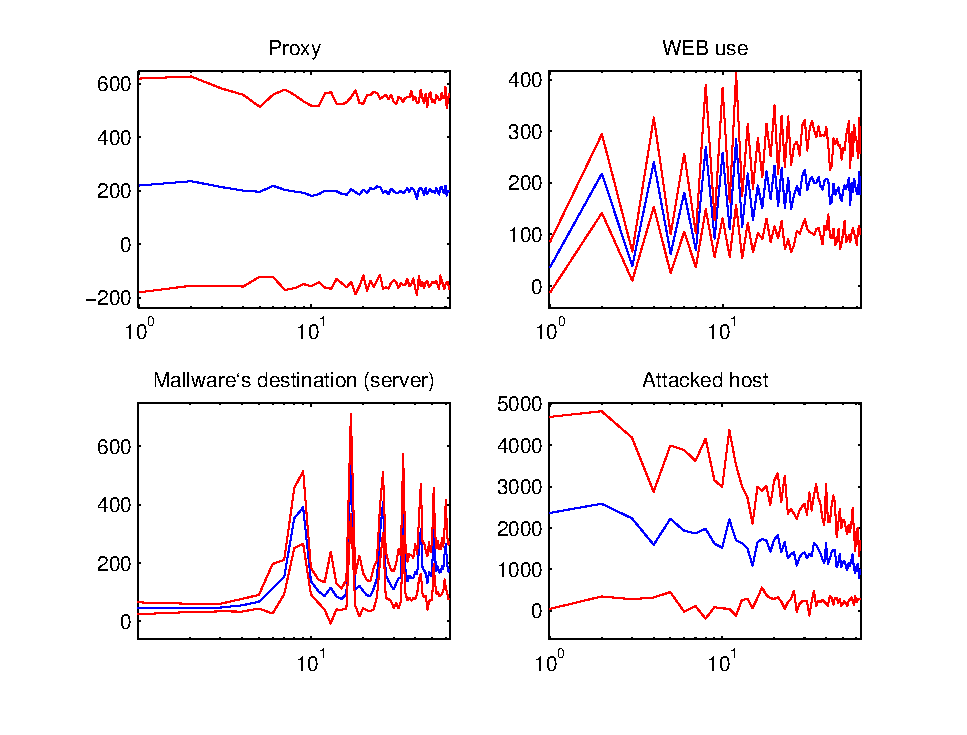
\includegraphics[width=150mm]{spect_dst_bdivp}
  \caption{Spectrums ($mean$ - blue, $mean\pm st.dev$ - red) of some  endpoints using feature $r_t^{(1)}$ and agregation over \textbf{target}}
  \label{fig:spect_dst_bdivp}
\end{figure}
\begin{figure}[t!]%
  \centering
  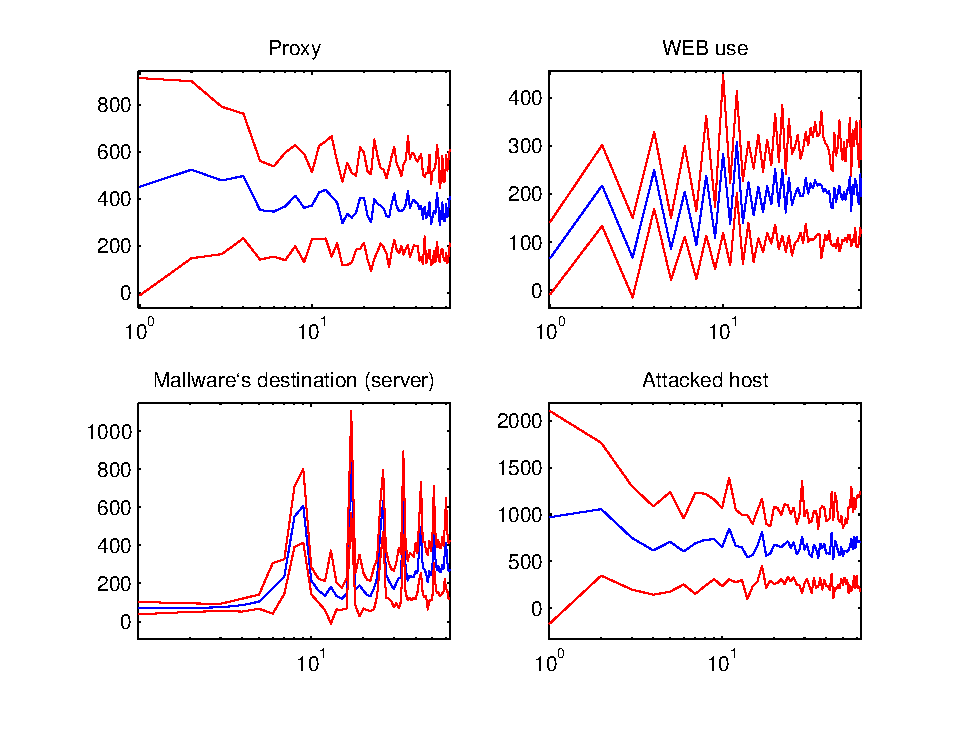
\includegraphics[width=150mm]{spect_src_bdivp}
  \caption{Spectrums ($mean$ - blue, $mean\pm st.dev$ - red) of some  endpoints using feature $r_t^{(1)}$ and agregation over \textbf{source}}
  \label{fig:spect_src_bdivp}
\end{figure}
\begin{figure}[t!]%
  \centering
  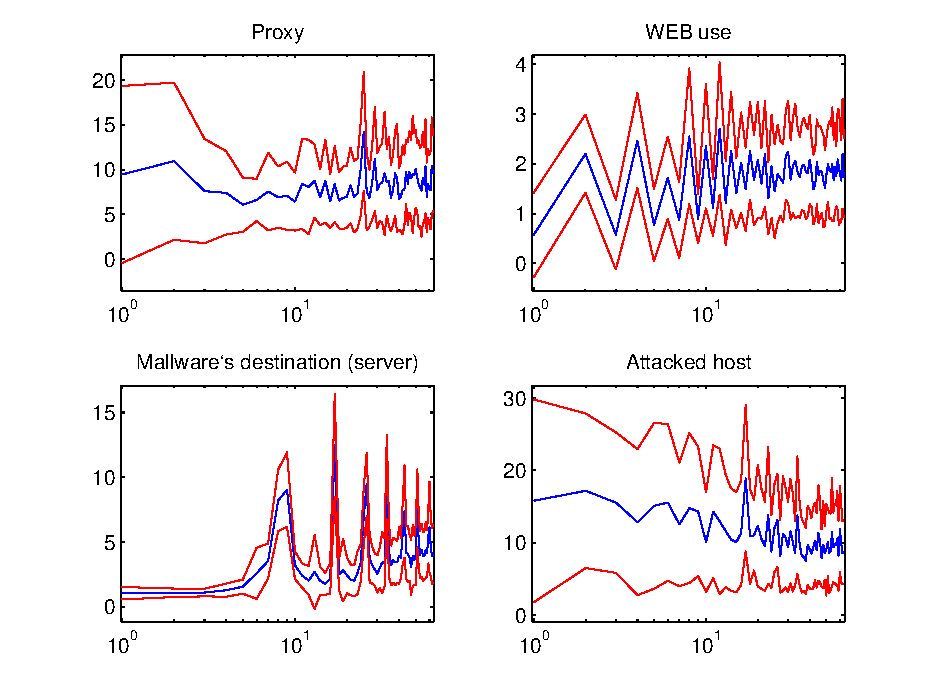
\includegraphics[width=150mm]{spect_dst_logp}
  \caption{Spectrums ($mean$ - blue, $mean\pm st.dev$ - red) of some  endpoints using feature $r_t^{(2)}$ and agregation over \textbf{target}}
  \label{fig:spect_dst_logp}
\end{figure}
\begin{figure}[t!]%
  \centering
  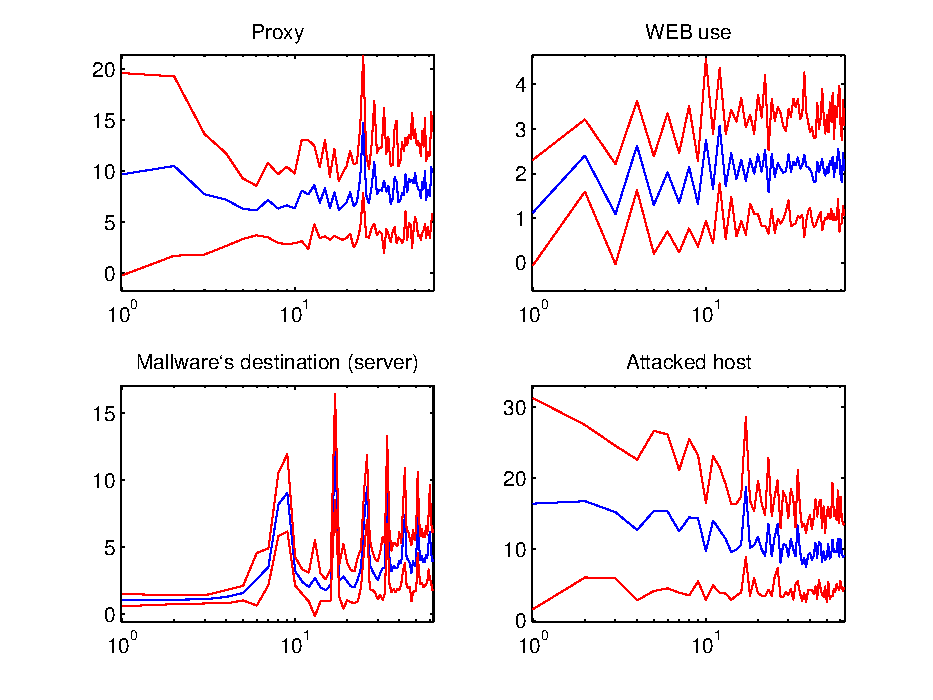
\includegraphics[width=150mm]{spect_src_logp}
  \caption{Spectrums ($mean$ - blue, $mean\pm st.dev$ - red) of some  endpoints using feature $r_t^{(2)}$ and agregation over \textbf{source}}
  \label{fig:spect_src_logp}
\end{figure}
\begin{figure}[t!]%
  \centering
  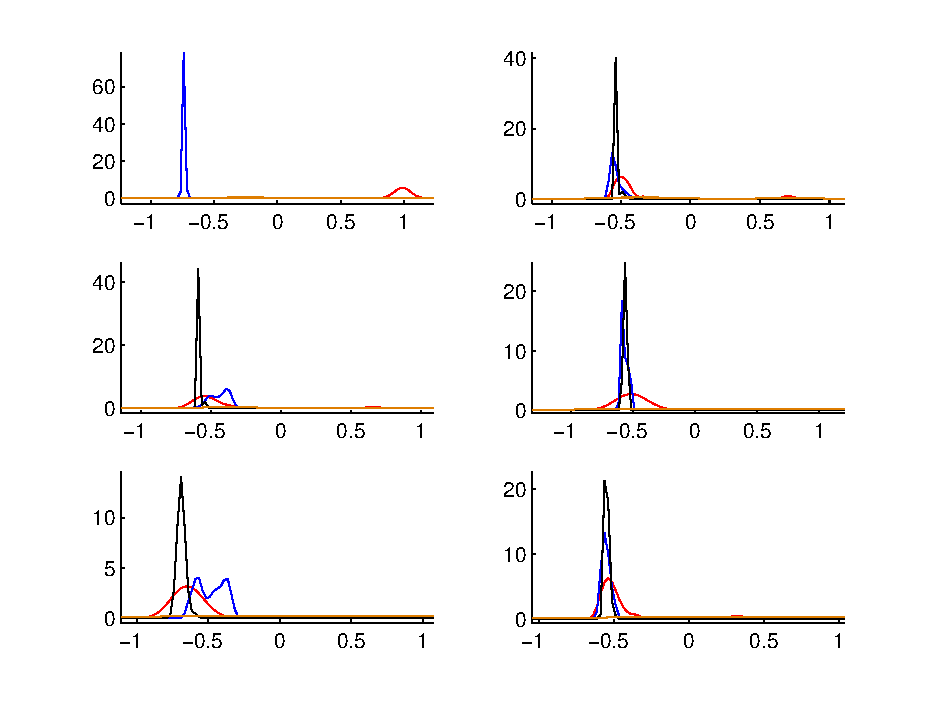
\includegraphics[width=140mm]{dens_dst_bdivp}
      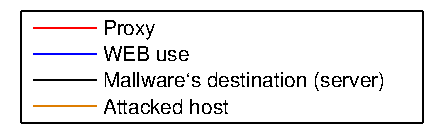
\includegraphics[width=40mm]{legend}
  \caption{Conditional probability $Pr(x|endpoint)$ density estimation (linear scaling ensuring zero global mean and global variance is 1)}
  \label{fig:dens_dst_bdivp}
\end{figure}
\begin{figure}[t!]%
  \centering
  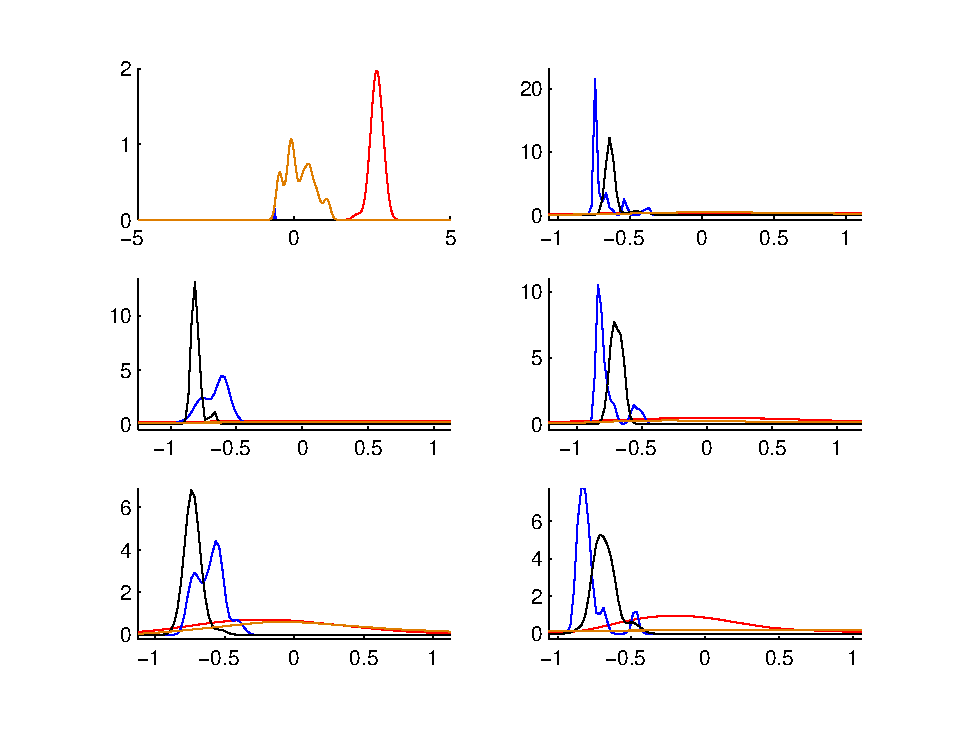
\includegraphics[width=140mm]{dens_dst_logp}
      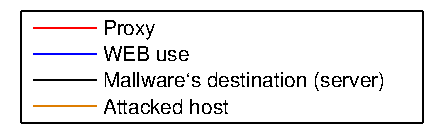
\includegraphics[width=40mm]{legend}
  \caption{Conditional probability $Pr(x|endpoint)$ density estimation (linear scaling ensuring zero global mean and global variance is 1)}
  \label{fig:dens_dst_logp}
\end{figure}
\begin{figure}[t!]%
  \centering
  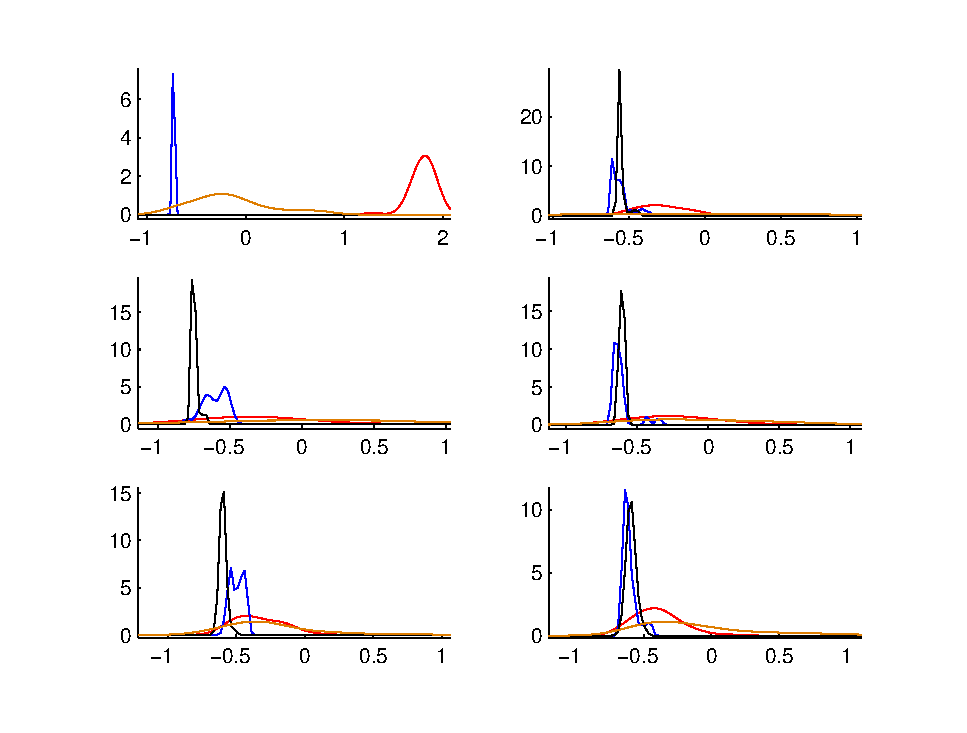
\includegraphics[width=140mm]{dens_src_bdivp}
    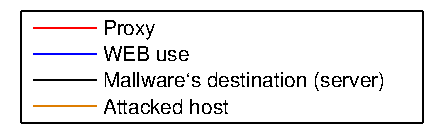
\includegraphics[width=40mm]{legend}
  \caption{Conditional probability $Pr(x|endpoint)$ density estimation (linear scaling ensuring zero global mean and global variance is 1)}
  \label{fig:dens_src_bdivp}
\end{figure}
\begin{figure}[t!]%
  \centering
  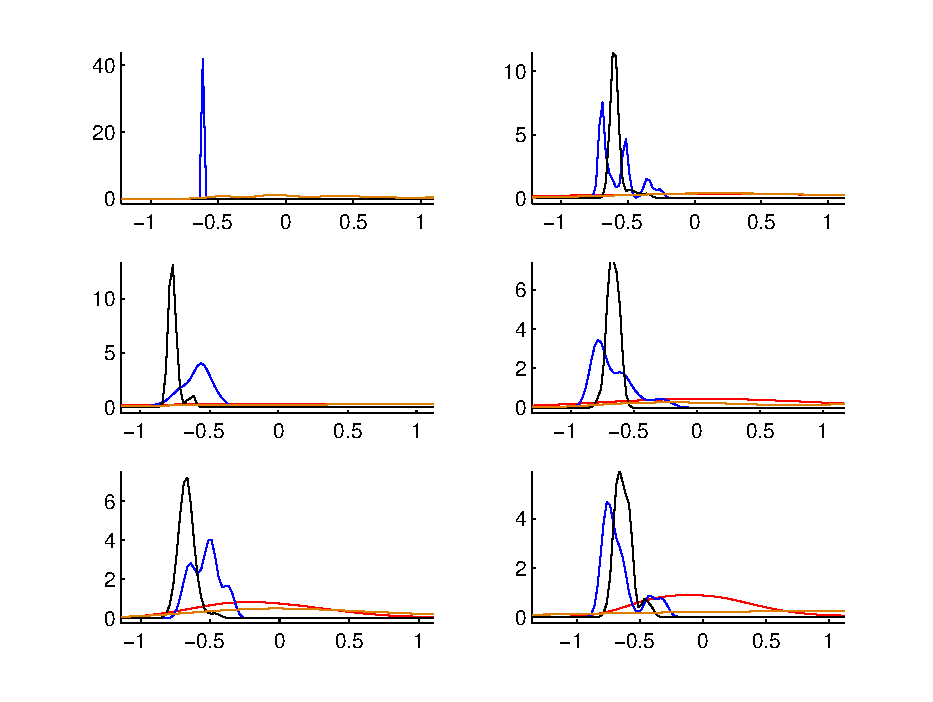
\includegraphics[width=140mm]{dens_src_logp}
  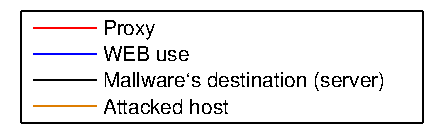
\includegraphics[width=40mm]{legend}
  \caption{Conditional probability $Pr(x|endpoint)$ density estimation (linear scaling ensuring zero global mean and global variance is 1)}
  \label{fig:dens_src_logp}
\end{figure}
\begin{figure}[t!]%
  \centering
  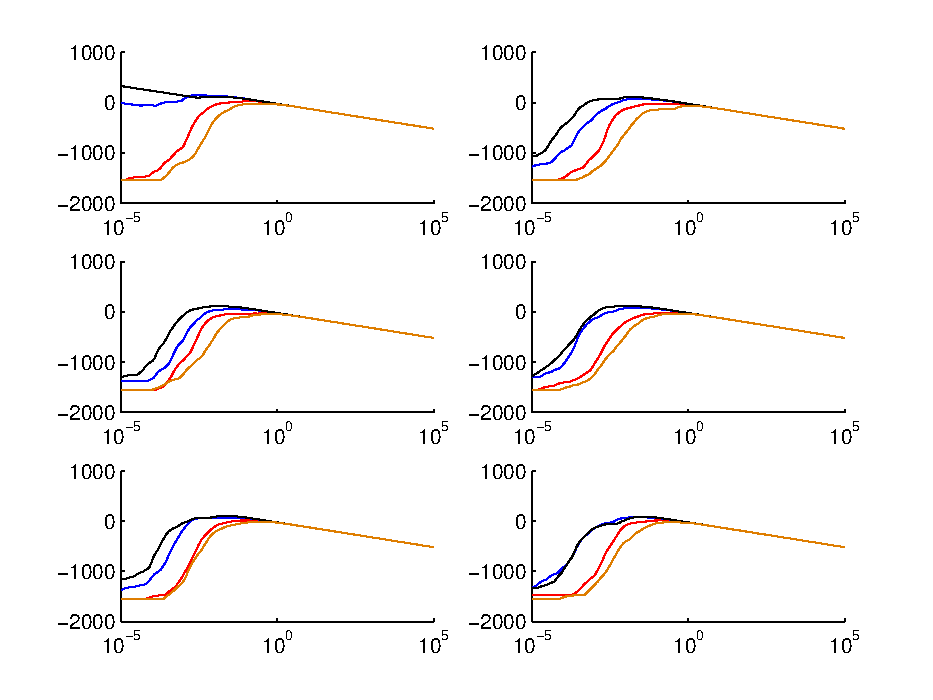
\includegraphics[width=140mm]{loglik_src_bdivp}
  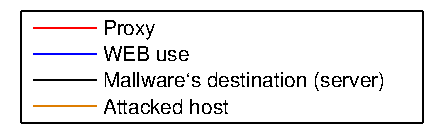
\includegraphics[width=40mm]{legend}
    \caption{Example of logarithmic likelihood $\log(L)$ (maximum likelihood estimation of the kernel width of the parzen window)}
  \label{fig:loglik_src_bdivp}
\end{figure}


%\begin{figure*}[!h] %
%  \centering
%  \subfloat[PCA projection]{\label{fig:som_topol_proj_7}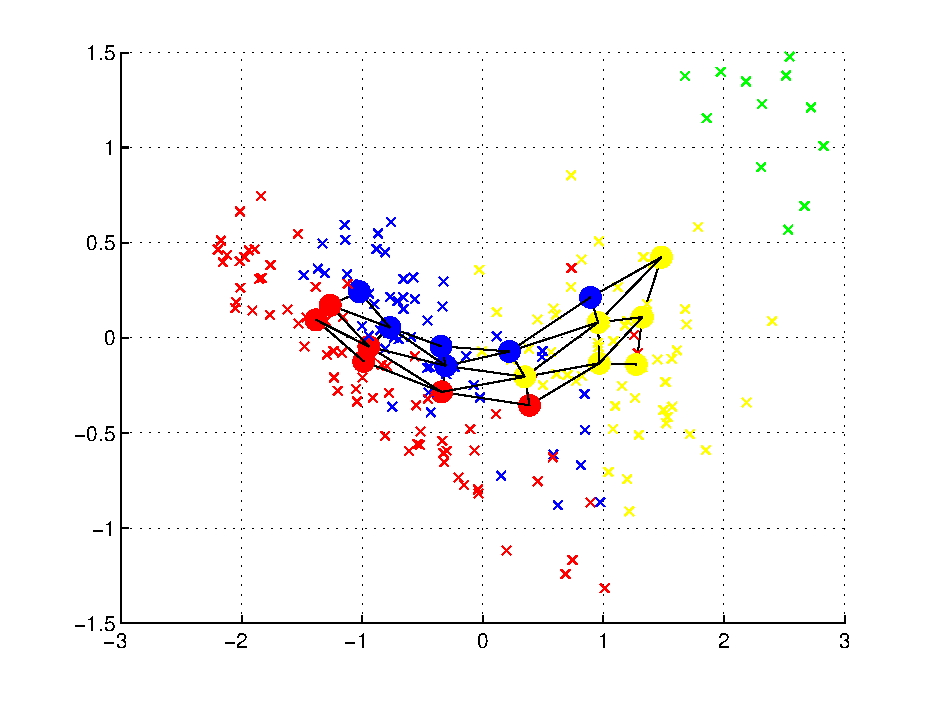
\includegraphics[width=55mm]{som_topol_proj_7}}
%  \subfloat[Sammon projection]{\label{fig:som_samon_proj_7}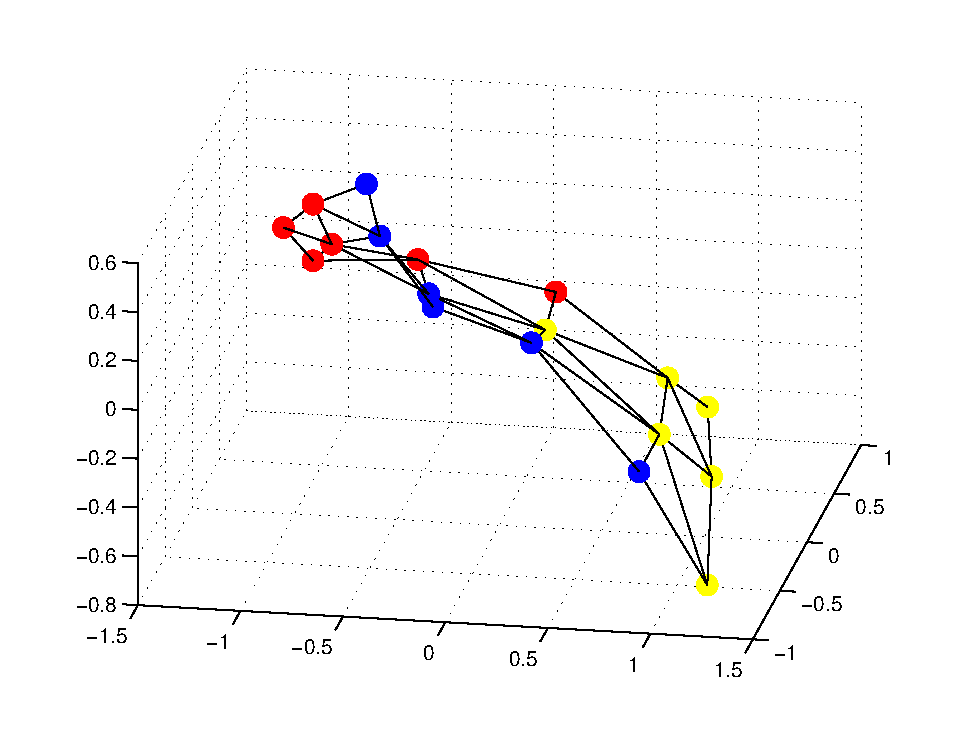
\includegraphics[width=55mm]{som_samon_proj_7}}
%  \subfloat[U-matrix and classification]{\label{fig:som_umat_7}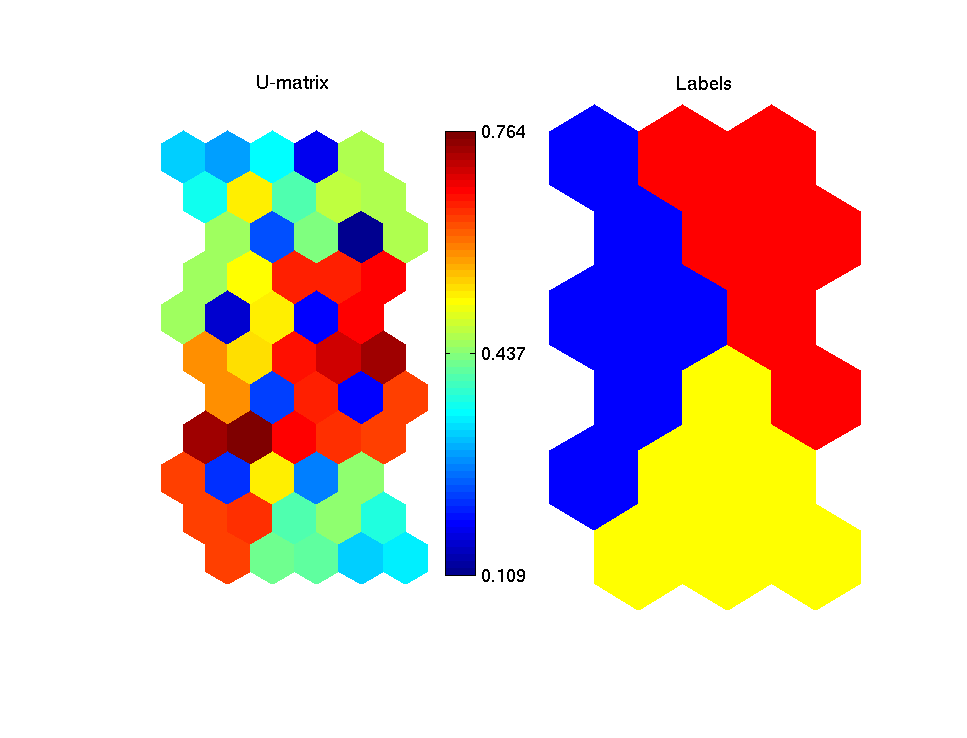
\includegraphics[width=55mm]{som_umat_7}}
%  \caption{configuration \#7 (see \textit{tbl. \ref{tbl:somresults}})}
%  \label{fig:som_config_7}
%\end{figure*}

% that's all folks
\end{document}
